\section{Sinchroninės (angl. “synchronous”) integracijos}

\subsection{Sinchroninių integracijų principas}
Sinchroninės integracijos dar gali būti apibūdinamos kaip „dviejų žmonių komunikavimas realiu laiku“ \cite{Bk6}. Su sinchroniniais komunikavimo pavyzdžiais dažnai susiduriame visi. Vienas iš tokių yra apsilankymas paprastoje internetinėje svetainėje.
Interneto naršyklėje suvedus puslapio pavadinimą, HTTP protokolo pagalba, mums iš serverio yra užkraunamas svetainės turinys ir atvaizduojamas.
Šis komunikavimo būdas yra paremtas užklausos/atsakymo (angl. \textit{„request/response“}) principu. Šiame modelyje egzistuoja
Klientas (tai yra mūsų naršyklė) ir serveris (tai yra interneto svetainės savininkas arba įmonė teikianti svetainių talpinimo paslaugas).
Klientas siunčia užklausą serveriui prašydamas resurso, šiuo atveju tai yra mūsų norimos pamatyti svetainės turinio, ir laukia kol svetainė atiduos atsakymą į užklausą.
Serveris reaguodamas į kliento užklausą grąžina atsakymą, kuris būti arba svetainės turinys, arba grąžinama klaida, pavyzdžiui kad toks resuras neegzistuoja arba 
klientas yra neautorizuotas šios svetainės lankytojas. Šis bendravimas yra perteiktas pateikta schema (\ref{img:synchronous-model} pav.):

\begin{figure}[H]
  \centering
  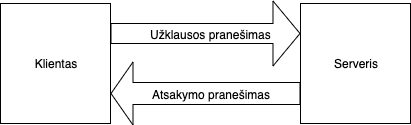
\includegraphics[scale=0.6]{img/synchronous-model}
  \caption{Sinchroninio komunikavimo schema.}
  \label{img:synchronous-model}
\end{figure}

Taigi šis modelis puikiai gali veikti ir mikroservisų sistemoje. Vienas servisas siunčia užklausą į kitą servisą norėdamas gauti
informaciją arba inicijuoti, kokį nors veiksmą. Šis modelis ypatingas tuo, kad yra primityvus ir iškart užklausą išsiuntęs servisas
žinos ar sėkmingai pavyko atlikti norimą veiksmą. Šis modelis yra labai geras, kai tik įvykus sėkmingai užklausai leidžiame vartotojui vykdyti
kitas operacijas ir kitaip bendrauti su mūsų sistema, tai yra vartotojo autentifikacija ir autorizacija.

Siekant geriau išaiškinti, kaip veikia sinchroninis komunikavimas mikroservisų sistemose, pateikiama modelinė situacija, kur komunikavimas vyktų būtent
minėtu būdu. Įsivaizduokime, kad egzistuoja universiteto informacinė sistema, kuri yra suprojektuota pasiremiant mikroservisų
architektiniu modeliu. Šioje sistemoje yra atskiri servisai atsakingi už studentų duomenų tvarkymą, dokumentų generavimą, elektroninių laiškų siuntimą, tvarkaraščių sudarymą 
ir saugojimą. Be šių servisų sistema turėtų turėti ir daug kitos paskirties mikroservisų, bet dabar aptarsime tik šiuos.
Taigi, sinchroniniu komunikavimo modeliu servisas atsakingas už studentų duomenų tvarkymą bus informuotas apie naujo studento kūrimo inicijavimą.
Šis servisas savo duomenų bazėje sukuria naują įrašą ir vykdo tokius veiksmus eilės tvarka:

\begin{enumerate}
  \item Siunčiama užklausa į dokumentų generavimo servisą, kad būtų gauti sugeneruoti aktai apie naujo studento užregistravimą sistemoje, ir laukiama atsakymo. Dokumentų servisas sugeneravęs dokumentą grąžintų atsakymą apie sėkmingą
  dokumento sugeneravimą.
	\item Gavus atsakymą iš dokumentų serviso, siunčiama užklausa į tvarkaraščių generavimo servisą ir laukiama atsakymo. Tvarkaraščių generavimo servisas formuoja studento tvarkaraštį ir grąžina atsakymą apie sėkmingą resurso sukūrimą.
	\item Po sėkmingo tarkaraščio sugeneravimo siunčiama užklausą į elektroninių laiškų servisą, siekiant informuoti naujo studento būsimus dėstytojus apie
  naują užsiėmimų dalyvį. Elektroninių laiškų servisas išsiuntęs visus laiškus grąžina atsakymą apie sėkmingai užbaigtą darbą.
  \item Be sistemos sutrikimų sėkmingai įvykdžius visus procesus, servisas atsakingas už studentų duomenų tvarkymą užbaigia naujo studento kūrimo procesą.
\end{enumerate}

Tokią veiksmų seką vaizdžiai parodo tokia ši schema, kur veiksmai vyksta paeiliui, o ne lygiagrečiai (\ref{img:synchronous-microservices-scheme} pav.):

\begin{figure}[H]
  \centering
  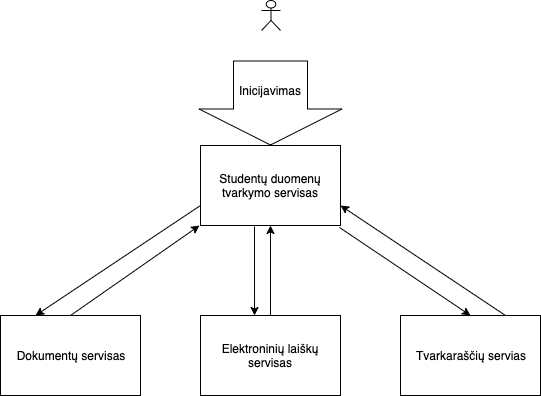
\includegraphics[scale=0.6]{img/synchronous-microservices-scheme}
  \caption{Sinchroninio komunikavimo mikroservisuose schema.}
  \label{img:synchronous-microservices-scheme}
\end{figure}

\subsection{Sinchroninių integracijų technologijos}
Būdų realizuoti sinchroninius komunikavimo modelius yra daug. Šiuo metu populiariausi yra du:
\begin{itemize}
	\item RESTful saityno tarnybos.
	\item SOAP saityno tarnybos.
\end{itemize}
\break

Turint omenyje, kad REST yra tik architektūrinis stilius, o ne protokolas, ir ju nelabai galima lyginti \cite{Misc5}. Tačiau
remiantis Joni Makkonen magistrinio darbo „REST ir SOAP saityno tarnybų efektyvumo ir naudojamumo palyginimas“ \cite{MstrThs2} galima teigti, kad
REST yra pranašesne ir šiame darbe išsiplėsime tik su šiuo architektūriniu stilium.
\break

REST saityno tarnybos užklausos struktūra yra paprasta. Ji susideda iš keletos atributų:
\begin{itemize}
	\item HTTP metodo, pvz.: \textit{„GET“, „POST“, „PUT“, „DELETE“}.
	\item Unikalaus resurso identifikatoriaus (arba adreso), pvz.: \textit{„http://mif.vu.lt/“}.
	\item Antraščių (angl. \textit{„Headers“}), pvz.: \textit{„Content-Type: application/json“}.
	\item Užklausos turinio (čia gali būti bet koks standartinis formatas, pvz.: \textit{„JSON“}).
	\item HTTP protokolo versija, pvz.: \textit{„HTTP/1.1“}.
\end{itemize}

REST atsakymo struktūra skiriasi nuo užklausos tik tuo, kad vietoje HTTP metodo, gaunamas HTTP statuso kodas. Tokio komunikavimo
per REST saityno tarnybas pavyzdį galime pamatyti šioje schemoje (\ref{img:Restful-scheme} pav.):

\begin{figure}[H]
  \centering
  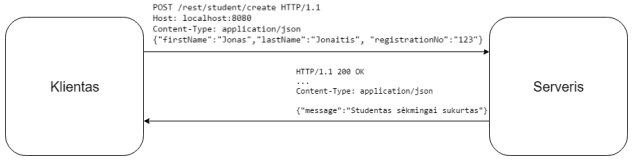
\includegraphics[scale=0.6]{img/Restful-scheme}
  \caption{REST saityno tarnybų schema.}
  \label{img:Restful-scheme}
\end{figure}

